\documentclass[
    table,
    12pt,
    oneside,
    a4paper,
    italian
]{book}

\PassOptionsToPackage{dvipsnames}{xcolor} % colori PDF/A

\usepackage{colorprofiles}
% PDF/A
% validate in https://www.pdf-online.com/osa/validate.aspx
\usepackage[a-1a,mathxmp]{pdfx}[2018/12/22]
\usepackage[T1]{fontenc}
\usepackage[utf8]{inputenc}
\usepackage[italian]{babel}
\usepackage{bookmark}
\usepackage{caption}
\usepackage{comment}
\usepackage{chngpage, calc} % centra il frontespizio
\usepackage{emptypage} % pagine vuote senza testatina e piede di pagina
\usepackage{epigraph} % per epigrafi
\usepackage{indentfirst} % rientra il primo paragrafo di ogni sezione
\usepackage{graphicx} % immagini
\usepackage[pdfa]{hyperref} % collegamenti ipertestuali
\usepackage{mparhack,relsize}  % finezze tipografiche
\usepackage{nameref} % visualizza nome dei riferimenti
\usepackage[font=small]{quoting} % citazioni
\usepackage{subfig} % sottofigure, sottotabelle
\usepackage[italian]{varioref} % riferimenti completi della pagina
\usepackage{longtable} % tabelle su più pagine
\usepackage[toc, acronym, automake]{glossaries}
\usepackage[backend=biber, style=verbose-ibid, hyperref, backref]{biblatex}
\usepackage{lmodern}
\usepackage[top=2.75cm, bottom=2.75cm, right=3cm, left=3.75cm]{geometry} % 1in+17pt+0.6cm
\usepackage{fancyhdr}
\usepackage{lipsum}
\usepackage{setspace}
\usepackage{titlesec}
\usepackage[cachedir=minted-caches]{minted} % https://it.overleaf.com/learn/latex/Code_Highlighting_with_minted
\usepackage{xcolor}
\usepackage{csquotes} % gestisce automaticamente i caratteri (")
\usepackage{etoolbox}
\usepackage[bottom]{footmisc}
\usepackage{zref-totpages}
% Load variables
\newcommand{\myUni}{Università degli Studi di Padova}
\newcommand{\myDepartment}{Dipartimento di Matematica ``Tullio Levi-Civita''}
\newcommand{\myFaculty}{Corso di Laurea in Informatica}
\newcommand{\myTitle}{Excelgen: generazione automatica della reportistica nei più comuni formati documentali}
\newcommand{\myDegree}{Tesi di Laurea Triennale}
\newcommand{\profTitle}{Prof.}
\newcommand{\myProf}{Ranzato Francesco}
\newcommand{\graduateTitle}{Laureando}
\newcommand{\myName}{Destro Stefano}
\newcommand{\myStudentID}{1229139}
\newcommand{\myAA}{2023-2024}
\newcommand{\myLocation}{Padova}
\newcommand{\myTime}{Settembre 2024}
% Acronyms
\newacronym{api}{API}{Application Program Interface}
\newacronym{sdk}{SDK}{Software Development Kit}
\newacronym{uml}{UML}{Unified Modeling Language}
\newacronym{tsa}{TSA}{Termine solo acronimo}
\newacronym{mvc}{MVC}{Model View Controller}
\newacronym{drf}{DRF}{Django REST Framework}
\newacronym{orm}{ORM}{Object-Relational Mapping}
\newacronym{dom}{DOM}{Document Object Model}
\newacronym{pmi}{PMI}{piccole e medie imprese}

% Glossary
\newglossaryentry{apig}{
    name={API},
    text={Application Program Interface},
    sort=api,
    description={In informatics, an API is a set of procedures available to programmers, typically grouped to form a toolkit for a specific task within a program. Its purpose is to provide an abstraction, usually between hardware and the programmer or between low-level and high-level software, simplifying the programming process}
}

\newglossaryentry{sdkg}{
    name={SDK},
    text={Software Development Kit},
    sort=sdk,
    description={A Software Development Kit (SDK) is a collection of development tools in one installable package, facilitating application creation by providing a compiler, debugger, and sometimes a software framework. SDKs are typically specific to a hardware platform and operating system combination. Many application developers use specific SDKs to enable advanced functionalities such as advertisements, push notifications, etc}
}

\newglossaryentry{umlg}{
    name={UML},
    text={Unified Modeling Language},
    sort=uml,
    description={In software engineering, Unified Modeling Language (UML) is a modeling and specification language based on the object-oriented paradigm. UML serves as a "lingua franca" in the object-oriented design and programming community. Much of the industry literature uses UML to describe analytical and design solutions in a concise and understandable way for a broad audience}
}

\newglossaryentry{TermineSenzaAcronimo}{
    name={Nome del termine},
    sort=termine senza acronimo,
    description={Descrizione}
}

\newglossaryentry{ormg}{
	name={ORM},
	sort=orm,
	text={Object-Relational Mapping},
	description={Tecnica di programmazione che permette di interagire con un database relazionale utilizzando oggetti di programmazione anziché scrivere direttamente query SQL. L'ORM mappa le classi del linguaggio di programmazione ai modelli del database, consentendo di manipolare i dati del database attraverso metodi e proprietà degli oggetti, semplificando la gestione delle operazioni di Create, Read, Update, Delete}
}

\newglossaryentry{domg}{
	name={DOM},
	sort=dom,
	text={Document Object Model},
	description={Rappresentazione ad albero di un documento HTML o XML, permette ai linguaggi di programmazione di manipolare la struttura, il contenuto e lo stile di una pagina web in modo dinamico}
}

\newglossaryentry{virtdom}{
	name={Virtual DOM},
	sort=virtdom,
	text={Virtual Document Object Model},
	description={copia leggera e in-memory del DOM reale, utilizzata principalmente da librerie come React per ottimizzare le operazioni di aggiornamento dell'interfaccia utente. Le modifiche vengono fatte sul Virtual DOM, e solo le differenze rispetto al DOM reale vengono applicate, migliorando così l'efficienza del rendering}
}

\newglossaryentry{pip}{
	name={pip},
	sort=pip,
	text={pip},
	description={Gestore di pacchetti ufficiale di Python, usato per installare, aggiornare e rimuovere pacchetti e librerie. Gestisce le dipendenze e facilita l'integrazione di nuovi pacchetti nei progetti Python}
}

\newglossaryentry{queryset}{
	name={QuerySet},
	sort=queryset,
	text={QuerySet},
	description={rappresentazione astratta di una query al database che restituisce una collezione di oggetti del modello su cui è stato invocato. È valutato in modo \textit{lazy}, consentendo di costruire e filtrare dinamicamente le query senza eseguire nell'immediato le operazioni sul database. I QuerySet supportano operazioni come filtraggio, ordinamento e aggregazione.}
}

\newglossaryentry{playground}{
	name={playground},
	sort=playground,
	text={playground},
	description={ambiente semplificato e isolato che emula le funzionalità di un sistema reale per consentire lo sviluppo, la sperimentazione di codice senza effetti collaterali su sistemi di produzione. Questi ambienti sono utilizzati per simulare scenari, verificare il comportamento di software e provare nuove idee in un contesto controllato e sicuro.}
}

\newglossaryentry{pandas}{
	name={Pandas},
	sort=Pandas,
	text={Pandas},
	description={libreria Python per l'analisi e la manipolazione di dati, offre strutture dati come DataFrame e Series. Fornisce funzionalità avanzate per l'elaborazione e l'analisi di dataset strutturati. Nell'ecosistema Django, Pandas può essere utilizzata efficacemente per elaborare i dati estratti dai modelli Django, trasformando queryset in DataFrame per analisi avanzate o per preparare i dati prima di renderizzarli o esportarli.}
}

% Define custom colors
\definecolor{hyperColor}{HTML}{0B3EE3}
\definecolor{tableGray}{HTML}{F5F5F7}
\definecolor{veryPeri}{HTML}{6667ab}

% Set line height
\linespread{1.5}

% Custom hyphenation rules
\hyphenation {
    data-base
    al-go-rithms
    soft-ware
}

% Images path
\graphicspath{{img/}}

% Force page color, as some editors set a grayish color as default
\pagecolor{white}

% Better spacing for footnotes
\setlength{\skip\footins}{5mm}
\setlength{\footnotesep}{5mm}

\setlength{\headheight}{14.5pt}
\addtolength{\topmargin}{-2.45pt}

% Add a subscript G to a glossary entry
\newcommand{\glox}{\textsubscript{\textbf{\textit{G}}}}

% Improvements the paragraph command
\titleformat{\paragraph}
{\normalfont\normalsize\bfseries}{\theparagraph}{1em}{}
\titlespacing*{\paragraph}
{0pt}{3.25ex plus 1ex minus .2ex}{1.5ex plus .2ex}

% Define use case environment
\newcounter{usecasecounter} % define a counter
\setcounter{usecasecounter}{0} % set the counter to some initial value
% Parameters
% #1: ID
% #2: Nome
\newenvironment{usecase}[2]{
    \renewcommand{\theusecasecounter}{\usecasename #1}  % this is where the display of the counter is overwritten/modified
    \refstepcounter{usecasecounter} % increment counter
    \vspace{2em}
    \par \noindent % start new paragraph
    {\normalsize \textbf{\usecasename #1: #2}} % display the title before the content of the environment is displayed
    \vspace{.5em}
}{
    \medskip
}
\newcommand{\usecasename}{UC}
\newcommand{\usecaseactors}[1]{\textbf{\\Attori Principali:} #1}
\newcommand{\usecasepre}[1]{\textbf{\\Precondizioni:} #1}
\newcommand{\usecasedesc}[1]{\textbf{\\Descrizione:} #1}
\newcommand{\usecasepost}[1]{\textbf{\\Postcondizioni:} #1}
\newcommand{\usecasealt}[1]{\textbf{\\Scenario Alternativo:} #1}

% Define risks environment
\newcounter{riskcounter} % define a counter
\setcounter{riskcounter}{0} % set the counter to some initial value
% Parameters
% #1: Title
\newenvironment{risk}[1]{
    \refstepcounter{riskcounter} % increment counter
    \par \noindent % start new paragraph
    \textbf{\arabic{riskcounter}. #1} % display the title before the content of the environment is displayed
}{
    \par\medskip
}
\newcommand{\riskname}{Rischio}
\newcommand{\riskdescription}[1]{\textbf{\\Descrizione:} #1.}
\newcommand{\risksolution}[1]{\textbf{\\Soluzione:} #1.}

% Apply fancy styling to pages
\pagestyle{fancy}
\fancyhf{}
\fancyhead[L]{\leftmark} % Places Chapter N. Chatper title on the top left
\fancyfoot[C]{\thepage} % Page number in the center of the footer

% Adds a blank page while increasing the page number
\newcommand\blankpage{ 
\clearpage
    \begingroup
    \null
    \thispagestyle{empty}
    \hypersetup{pageanchor=false}
    \clearpage
\endgroup
}

% Adds a blank page while increasing the page number
\newcommand\blankpagewithnumber{ 
  \clearpage
  \thispagestyle{plain} % Use plain page style to keep the page number
  \null
  \clearpage
}

% Increase page numbering
\newcommand\increasepagenumbering{
    \addtocounter{page}{+1}
}

% Make glossaries and bibliography
\makeglossaries
% Redefine the format for the glossary entries to be italic
\renewcommand*{\glstextformat}[1]{\textit{#1}\glox}
%\glsaddall

\bibliography{references/bibliography}
\defbibheading{bibliography} {
    \cleardoublepage
    \phantomsection
    \addcontentsline{toc}{chapter}{\bibname}
    \chapter*{\bibname\markboth{\bibname}{\bibname}}
}

% Code blocks handling w/ table of codes
\makeatletter
\ifdefined\NR@chapter
  \expandafter\@firstoftwo
\else
  \expandafter\@secondoftwo
\fi{\patchcmd\NR@chapter}{\patchcmd\@chapter}
  {\addtocontents{lot}{\protect\addvspace{10\p@}}}
  {\addtocontents{lot}{\protect\addvspace{10\p@}}%
   \addtocontents{lol}{\protect\addvspace{10\p@}}}
  {}{}
\makeatother

\renewcommand\listingscaption{Codice}
\renewcommand\listoflistingscaption{Elenco dei codici sorgenti}
\counterwithin*{listing}{chapter}
\renewcommand\thelisting{\thechapter.\arabic{listing}}

% Set up hyperlinks
\hypersetup{
    colorlinks=true,
    linktocpage=true,
    pdfstartpage=1,
    pdfstartview=,
    breaklinks=true,
    pdfpagemode=UseNone,
    pageanchor=true,
    pdfpagemode=UseOutlines,
    plainpages=false,
    bookmarksnumbered,
    bookmarksopen=true,
    bookmarksopenlevel=1,
    hypertexnames=true,
    pdfhighlight=/O,
    allcolors = hyperColor
}

% Set up captions
\captionsetup{
    tableposition=top,
    figureposition=bottom,
    font=small,
    format=hang,
    labelfont=bf
}

% When draft mode is on, the hyperlinks are removed. Useful when printing the document. To enable/disable, uncomment/comment the command
% \hypersetup{draft}

% prevents cleaning up the cache at the end of the run (needed to keep the unused caches, generated by other editions)
\makeatletter
\renewcommand*{\minted@cleancache}{}
\makeatother

% Break lines in code blocks whe using inputminted
\setminted{breaklines}

\date{}

\hypersetup{pdfstartview=}
\begin{document}
    \frontmatter
    \begin{titlepage}
    \begin{center}
        \begin{Large}
            \textbf{\myUni}\\
        \end{Large}

        \vspace{5pt}

        \begin{large}
            \textsc{\myDepartment}\\
        \end{large}

        \vspace{5pt}

        \begin{large}
            \textsc{\myFaculty}\\
        \end{large}

        \vspace{25pt}
        
        \begin{figure}[htbp]
            \centering
            
\includegraphics[alt={Emblema dell'Università degli Studi di Padova}, height=6cm]{img/logo_unipd.jpeg}
        \end{figure}

        
        \begin{Large}
            \textbf{\myTitle}\\
        \end{Large}

        \vspace{5pt}

        \begin{large}
            \textit{\myDegree}\\
        \end{large}

        \vspace{50pt}
        
        \begin{normalsize}
            \begin{flushleft}
                \textit{Relatore}\\
                \profTitle\ \myProf
            \end{flushleft}

            \vspace{-48pt}
            
            \begin{flushright}
                \textit{\graduateTitle}\\
                \myName\\
                Matricola \myStudentID
            \end{flushright}
        \end{normalsize}

        \vspace*{\fill}
        
        \line(1, 0){338} \\
        \begin{normalsize}
            \textsc{Anno Accademico \myAA}
        \end{normalsize}
    \end{center}
\end{titlepage}

    \increasepagenumbering % increase the page numbrering by 1, in order to cout the frontispiece
    \clearpage
\phantomsection
\thispagestyle{empty}
\hfill
\vfill

{\small\noindent\textcopyright\ \myName, \myTime. Tutti i diritti riservati. \myDegree: ``\textit{\myTitle}'', \myUni, \myDepartment.}
    \cleardoublepage
\phantomsection
\pdfbookmark{Ringraziamenti}{Ringraziamenti}

\begin{flushright}{
    \slshape
    ``Colui il quale ha inseguito e sconfitto i demoni Sem, che ora vagano per il mondo, domandandosi: «ma nü, chi sëm?»''} \\
    \medskip
    --- Il grande Pdor, figlio di Kmer, della tribù di Ishtar, della terra desolata dei Kfnir, uno degli ultimi sette saggi: Pfulur, Galér, Astaparigna, Sùsar, Param, Fusus e Tarìm.
\end{flushright}

\begingroup
\let\clearpage\relax
\let\cleardoublepage\relax
\let\cleardoublepage\relax

\chapter*{Ringraziamenti}

\noindent Desidero esprimere la mia gratitudine al professor \myProf, mio relatore, per l'aiuto e il sostegno che mi ha dato durante la stesura dell'elaborato.

\vspace{0.35cm}

\noindent Vorrei anche ringraziare, con affetto, i miei genitori per il loro sostegno, il grande aiuto e la loro presenza in ogni momento durante gli anni di studio.

\vspace{0.35cm}

\noindent Desidero poi ringraziare i miei amici per i bellissimi anni trascorsi insieme e le mille avventure vissute.

\vspace{0.75cm}

\noindent{\myLocation, \myTime}
\hfill \textit{\myName}

\endgroup

    \cleardoublepage
\phantomsection
\pdfbookmark{Compendio}{Compendio}
\begingroup
\let\clearpage\relax
\let\cleardoublepage\relax
\chapter*{Sommario}

Il presente documento descrive il lavoro svolto durante il periodo di stage, \lipsum[1]

\endgroup
\vfill

    \cleardoublepage
\pdfbookmark{\contentsname}{tableofcontents}
\setcounter{secnumdepth}{5}
\setcounter{tocdepth}{5}     

\tableofcontents
\clearpage

\begingroup
    \let\clearpage\relax
    \let\cleardoublepage\relax
    \let\cleardoublepage\relax

    % Figures list
    \phantomsection
    \pdfbookmark{\listfigurename}{lof}
    \listoffigures
    \vspace*{8ex}

    % Tables list
    \phantomsection
    \pdfbookmark{\listtablename}{lot}
    \listoftables
\endgroup

\begingroup
    % Code list
    \phantomsection
    \pdfbookmark{\listoflistingscaption}{lol}
    \listoflistings
\endgroup

\cleardoublepage
    \printglossary[type=\acronymtype, title=Acronimi e abbreviazioni, toctitle=Acronimi e abbreviazioni]
    \printglossary[type=main, title=Glossario, toctitle=Glossario]
    \blankpage % example of a blank page that also increases the page couter by 1

    \mainmatter
    \chapter{RiskApp}
\label{chap:introduzione}



\section{Storia}
Fondata nel 2015 da un gruppo di studenti dell'Università Ca' Foscari di Venezia, RiskApp (logo in figura \ref{fig:riskapp}) è una \textit{startup insurtech} con sede a Conselve, in provincia di Padova. La società si è rapidamente affermata nel settore della trasformazione digitale e dell'analisi avanzata del rischio per il comparto assicurativo.

\begin{figure}[H]
	\centering
	
\includegraphics[alt={Logo docx, xlsx e pdf}, width=0.5\columnwidth]{img/riskapp_logo.png}
	\caption{Logo RiskApp}
	\label{fig:riskapp}
\end{figure}

\subsection{Insurance Advisor}
In parallelo a RiskApp opera Insurance Advisor, una società di consulenza assicurativa. Sebbene le due aziende mantengano una propria identità e un proprio campo d'azione, lavorano in sinergia per offrire un servizio completo ai propri clienti.
Insurance Advisor è una società di consulenza assicurativa che supporta privati e aziende nella scelta delle coperture assicurative più adatte alle loro specifiche necessità. L'approccio verso le aziende è altamente personalizzato e basato su un'analisi approfondita delle esigenze del cliente e su una consulenza indipendente.
Grazie alle soluzioni digitali di RiskApp, Insurance Advisor può offrire ai propri clienti un’analisi del rischio più precisa e basata su dati reali, migliorando così la qualità delle loro consulenze.

\section{Obiettivi}
L'azienda integra tecnologie avanzate come \textit{machine learning}, i \textit{big data} e il \textit{cloud computing} nelle sue soluzioni. Queste tecnologie permettono a RiskApp di offrire una gamma di servizi che supportano le compagnie assicurative e gli intermediari nel loro percorso di digitalizzazione e nella gestione delle esigenze assicurative delle \gls{pmi}. L'obiettivo di RiskApp è fornire strumenti che non solo migliorano l'efficienza operativa, ma che consentono anche una gestione proattiva e a 360 gradi del rischio, rendendo le aziende più resilienti di fronte agli imprevisti.

L'azienda ha sviluppato una piattaforma digitale avanzata che consente alle compagnie assicurative di migliorare i propri processi e agli intermediari di gestire con maggiore precisione e velocità le esigenze dei clienti.

\section{Clienti}
RiskApp offre una gamma di soluzioni che si rivolgono principalmente a due categorie di clienti:
\begin{itemize}
	\item \textbf{Compagnie assicurative:} RiskApp aiuta le compagnie assicurative nel processo di digitalizzazione anticipando per quanto possibile le richieste dei clienti;
	\item \textbf{Intermediari assicurativi:} la piattaforma fornisce strumenti di analisi utili per offrire consulenze più mirate e di individuare le coperture assicurative più adatte alle esigenze assicurative dei clienti.
\end{itemize}

\section{Piattaforme e tecnologie}
Al cuore delle soluzioni di RiskApp vi è una piattaforma tecnologica che sfrutta l'intelligenza artificiale per analizzare grandi quantità di dati e generare previsioni accurate sui rischi. Questa piattaforma è progettata per essere altamente scalabile e flessibile, in modo da poter essere adattata alle diverse esigenze delle compagnie assicurative e dei loro intermediari.

\begin{itemize}
	\item \textbf{Intelligenza artificiale e \textit{Big Data}:} RiskApp utilizza algoritmi avanzati di \textit{machine learning} per analizzare dati storici e attuali, identificando pattern che possono indicare potenziali rischi. Questo approccio permette di prevedere eventi come catastrofi naturali o variazioni significative nel mercato, consentendo ai clienti di adottare misure preventive efficaci;
	\item \textbf{\textit{Cloud Computing}:} la piattaforma di RiskApp è basata su un'infrastruttura \textit{cloud}, che garantisce un accesso sicuro e continuo ai dati e agli strumenti di analisi. Questo consente una gestione centralizzata e in tempo reale delle informazioni, facilitando la collaborazione tra le diverse parti coinvolte nel processo assicurativo;
	\item \textbf{Analisi in tempo reale}: la piattaforma consente il monitoraggio continuo delle variabili di rischio, offrendo aggiornamenti in tempo reale. Questa funzionalità è particolarmente utile per le \gls{pmi} che devono gestire rischi non statici e in continua evoluzione.
\end{itemize}

\subsection{Esperienza personale}
Data la mia esperienza in azienda, queste sono le tecnologie adottate che ho avuto modo di osservare:
\begin{itemize}
	\item \textbf{Computer:} nello specifico portatili Apple con il loro sistema operativo proprietario;
	\item \textbf{Microsoft Office 365:} servizio Microsoft in abbonamento, gli strumenti prevalentemente usati sono Word, Excel e Outlook;
	\item \textbf{Slack:} piattaforma analoga a Microsoft Teams, utile per le conversazioni interne all'azienda e per lo scambio veloce di allegati;
	\item \textbf{GitHub:} piattaforma di \textit{hosting} per progetti software basata su Git, che offre versionamento del codice, gestione collaborativa tramite \textit{pull request}, integrazione continua e un \textit{issue tracking system} per il monitoraggio di \textit{bug} e richieste;
	\item \textbf{PyCharm Professional:} IDE avanzato per lo sviluppo Python, con funzionalità di \textit{debug}, supporto per \textit{framework web} e strumenti di \textit{refactoring} e \textit{testing};
	\item \textbf{Jira:} una piattaforma di gestione dei progetti e \textit{issue tracking}, ampiamente utilizzata per il monitoraggio delle attività, la gestione dei \textit{bug} e la pianificazione agile, con strumenti di \textit{reporting} e integrazione continua;
	\item \textbf{Visual Studio Code:} editor di codice open-source estensibile, che supporta numerosi linguaggi di programmazione, offre debugging integrato, terminale, e un ricco ecosistema di estensioni;
	\item \textbf{Docker:} una piattaforma per la creazione e gestione di container, che consente agli sviluppatori di automatizzare la distribuzione delle applicazioni e garantire consistenza tra ambienti di sviluppo, \textit{testing} e produzione;
	\item \textbf{WebStorm Professional:} IDE per lo sviluppo JavaScript e TypeScript, con strumenti integrati per il debugging, il testing, il refactoring e il supporto avanzato per framework front-end come React.
\end{itemize}

RiskApp per sviluppare i suoi applicativi usa più linguaggi di programmazione, \textit{framework} e librerie in base alle proprie necessità.

Le principali tecnologie per \textit{frontend} e \textit{backend} che ho avuto modo di vedere e/o discutere sono:
\begin{itemize}
	\item \textbf{Django:} framework web in Python che facilita lo sviluppo rapido di applicazioni, fornendo un'architettura \gls{mvc}, gestione dei database tramite \gls{ormg}, autenticazione e pannello di amministrazione integrati;
	\item \textbf{\gls{drf}:} toolkit per la creazione di API RESTful in Django, che include gestione delle autenticazioni, serializzazione dei dati e strumenti per il versionamento;
	\item \textbf{React:} libreria JavaScript per la costruzione di interfacce utente interattive e componenti riutilizzabili, basata su un modello a componenti e il concetto di \gls{virtdom} che gestisce le operazioni sul \gls{domg} per ottimizzare le prestazioni di rendering;
	\item  \textbf{Celery}: libreria Python per l'esecuzione asincrona di task distribuiti, spesso utilizzata con Django per gestire operazioni a lungo termine come invio di email, elaborazione di dati o operazioni di background.
\end{itemize} 

\subsection{Servizi offerti}
Insieme, RiskApp e Insurance Advisor offrono una gamma di servizi che copre tutte le fasi della gestione del rischio e della consulenza assicurativa:
\begin{itemize}
	\item \textbf{Analisi del rischio su misura:} RiskApp fornisce gli strumenti tecnologici per l'analisi dei dati e la previsione dei rischi, mentre Insurance Advisor si occupa di interpretare i dati e quindi consigliare le coperture assicurative più adeguate;
	\item \textbf{Gestione del rischio continuativa:} Questo servizio è particolarmente utile per le aziende che operano in settori ad alta volatilità o che sono esposte a rischi significativi, come quelli legati alle catastrofi naturali;
	\item \textbf{Consulenza assicurativa:} Insurance Advisor, offre una consulenza mirata supportando i clienti nella fase di scelta delle polizze. Questo approccio consente di ridurre i costi e di evitare coperture ridondanti o non necessarie;
	\item \textbf{Supporto post-vendita:} dopo la sottoscrizione delle polizze, viene offerto supporto nella gestione dei sinistri e nella revisione periodica delle coperture. La piattaforma di RiskApp fornisce dati aggiornati che possono essere utilizzati per rinegoziare i termini delle polizze o per adattare le coperture alle nuove condizioni di rischio.
\end{itemize}

\section{Organizzazione del testo}
\begin{description}
    \item[{\hyperref[chap:stage_desc]{Il secondo capitolo}}] descrive ...
    
    \item[{\hyperref[chap:descrizione-stage]{Il terzo capitolo}}] approfondisce ...
    
    \item[{\hyperref[chap:analisi-requisiti]{Il quarto capitolo}}] approfondisce ...
    
    \item[{\hyperref[chap:progettazione-codifica]{Il quinto capitolo}}] approfondisce ...
    
    \item[{\hyperref[chap:verifica-validazione]{Il sesto capitolo}}] approfondisce ...
    
    \item[{\hyperref[chap:conclusioni]{Nel settimo capitolo}}] descrive ...
\end{description}

Riguardo la stesura del testo, relativamente al documento sono state adottate le seguenti convenzioni tipografiche:
\begin{itemize}
	\item gli acronimi, le abbreviazioni e i termini ambigui o di uso non comune menzionati vengono definiti nel glossario, situato alla fine del presente documento;
	\item per la prima occorrenza dei termini riportati nel glossario viene utilizzata la seguente nomenclatura: \gls{domg};
	\item i termini in lingua straniera o facenti parti del gergo tecnico sono evidenziati con il carattere \textit{corsivo}.
\end{itemize}

\begin{listing}[H]
\begin{minted}{c}
#include <stdio.h>
int main() {
    print("Hello, world!");
    return 0;
}
\end{minted}
\caption{Example of code}
\label{listing:a}
\end{listing}

\newpage
    \chapter{Stage curricolare}
\label{chap:stage_desc}

\section{RiskApp e il rapporto con gli stage}
RiskApp vede negli stage un catalizzatore per l'innovazione e lo sviluppo aziendale. I tirocinanti, prossimi alla laurea triennale in informatica, possono portare conoscenza nelle tecnologie emergenti e l'abilità di esplorarle e applicarle. Pur rispettando i vincoli tecnologici aziendali, RiskApp incoraggia gli stagisti a introdurre soluzioni innovative nei progetti, consentendo così di valutarne i potenziali benefici e considerarne l'integrazione nei prodotti esistenti.

L'approccio di RiskApp mira a massimizzare il valore generato dagli stage. Il processo inizia con la selezione accurata di progetti che bilanciano complessità e rilevanza pratica e assicurandosi che questi rispondano a reali esigenze aziendali. Al termine del tirocinio, RiskApp organizza una sessione di confronto tra lo stagista e il team di sviluppo pertinente, facilitando uno scambio di idee sulle soluzioni implementate. Successivamente, l'azienda analizza approfonditamente il lavoro svolto dallo stagista, valutando l'implementazione delle innovazioni proposte nei prodotti esistenti.

Oltre al valore tecnico, gli stage fungono da efficace strumento di \textit{recruitment} per RiskApp. L'azienda identifica i tirocinanti più promettenti, in particolare quelli intenzionati a entrare nel mondo del lavoro dopo la laurea triennale. Questi candidati vengono considerati per potenziali opportunità di impiego, consentendo a RiskApp di arricchire il proprio organico con talenti già integrati nei processi e nella cultura aziendale.

Questo approccio \textit{multifaceted} agli stage permette a RiskApp di coltivare l'innovazione, migliorare i propri prodotti e attrarre nuovi talenti, creando un ciclo di crescita e sviluppo aziendale.

\section{Descrizione del progetto}
L'origine dello stage si radica in una necessità concreta di RiskApp: perfezionare e uniformare il proprio sistema di generazione di report. Nel suo ruolo di fornitore di soluzioni assicurative, RiskApp offre alla propria clientela la possibilità di accedere a report dettagliati in una varietà di formati, inclusi fogli di calcolo, documenti di testo e PDF. Questi report presentano una notevole diversità in termini di contenuto e struttura, riflettendo la specificità dei dati e dei servizi a cui si riferiscono.

Fino a questo momento, l'approccio adottato da RiskApp per gestire questa complessità si basava sull'utilizzo di script dedicati a casi specifici, talvolta anche isolati. Sebbene questa metodologia si sia dimostrata funzionale nel breve termine, ha evidenziato nel tempo significative limitazioni in termini di scalabilità ed efficienza operativa. In particolare, la necessità di apportare modifiche a cascata tra i vari script ha messo in luce l'esigenza di sviluppare una soluzione più flessibile e adattabile alle diverse esigenze.

\section{Obiettivi}
Lo scopo principale dello stage consiste nel progettare e sviluppare una libreria Python personalizzata, concepita per agevolare il processo di generazione della reportistica. Questa libreria, destinata all'utilizzo interno, sarà progettata per raccogliere e generalizzare le funzioni necessarie per generare reportistica in diversi formati.

Gli obiettivi specifici del progetto includono:

\begin{itemize}
	\item Creare una libreria flessibile che consenta il download agevole e automatizzato della reportistica nei formati XLSX, DOCX e PDF;
	\item garantire una gestione efficiente delle regole condizionali richieste;
	\item semplificare complessivamente il processo di generazione di report;
	\item rendere la libreria disponibile per l'installazione tramite il gestore di pacchetti \gls{pip}, facilitando così l'integrazione nelle attuali infrastrutture software dell'azienda.
\end{itemize}

\begin{figure}[H]
	\centering
	
\includegraphics[alt={Logo docx, xlsx e pdf}, width=1\columnwidth]{img/format_logos.jpg}
	\caption{Logo formati documentali supportati}
	\label{fig:logos}
\end{figure}

Questo progetto ambizioso si propone inoltre di raggiungere i seguenti risultati:

\begin{itemize}
	\item \textbf{Semplificazione del processo:} ridurre la complessità nella creazione dei report, eliminando la necessità di gestire molteplici script isolati;
	\item \textbf{Incremento dell'efficienza:} accelerare il processo di generazione di report per nuovi casi specifici;
	\item \textbf{Standardizzazione:} implementare un approccio uniforme alla generazione dei report, facilitando la manutenzione e l'aggiornamento delle modalità di \textit{reporting};
	\item \textbf{Flessibilità:} creare una soluzione adattabile a diverse tipologie di dati e requisiti di \textit{reporting}, riducendo la necessità di sviluppare soluzioni \textit{ad hoc} per ogni nuovo caso d'uso;
	\item \textbf{Scalabilità:} progettare un sistema in grado di crescere e adattarsi alla diversificazione dei servizi offerti;
	\item \textbf{Base per future innovazioni:} fornire una piattaforma su cui costruire future espansioni o cambiamenti.
\end{itemize}

La realizzazione di questa libreria Python rappresenta quindi un passo verso l'ottimizzazione dei processi interni di RiskApp. Questo progetto non solo mira a risolvere le sfide immediate legate alla generazione dei report, ma si configura anche come un investimento per il futuro dell'azienda. 

In conclusione, questo progetto di stage si colloca all'intersezione tra l'ottimizzazione dei processi interni e l'innovazione tecnologica, riflettendo l'impegno che RiskApp pone nel miglioramento continuo dei propri servizi e rispondendo più efficacemente alle esigenze in continua evoluzione dei propri clienti.

\section{Motivi della scelta dell'attività di stage}
Il mio percorso verso lo stage in RiskApp è stato caratterizzato da una serie di circostanze favorevoli e scelte ponderate. A differenza di molti miei colleghi, non ho partecipato all'evento StageIT, ma sono entrato in contatto con l'azienda attraverso un canale differente.

RiskApp, ha attirato la mia attenzione per diversi motivi. In primo luogo, la dimensione ridotta dell'azienda e il suo ambiente dinamico promettevano un'esperienza di stage stimolante e ricca di opportunità di apprendimento. L'età media giovane del team e l'atmosfera energica che ne derivava rappresentavano per me un valore aggiunto significativo.

Ciò che ha reso l'approccio con RiskApp particolarmente interessante è stato il fatto che l'azienda stessa mi ha contattato, dimostrando interesse. Questo approccio proattivo da parte loro ha sicuramente influenzato positivamente la mia percezione dell'azienda e ha contribuito a farmi sentire valorizzato fin dall'inizio.

Durante i colloqui successivi, ho avuto modo di approfondire diversi aspetti cruciali:

\begin{itemize}
	\item \textbf{Il progetto di stage:} mi è stata presentata un'opportunità che si allineava perfettamente con i miei interessi e le mie competenze. Il progetto prevedeva lo sviluppo con tecnologie backend, un'area che mi appassiona particolarmente per la sua enfasi sulla logica e sulla risoluzione di problemi anche complessi;
	\item \textbf{Le tecnologie utilizzate:} la possibilità di lavorare con Django, un framework che avevo già intenzione di approfondire, ha rappresentato un forte incentivo. Questa opportunità mi avrebbe permesso di consolidare le mie competenze in un ambito di grande rilevanza nel mercato del lavoro attuale;
	\item \textbf{Il personale:} durante i colloqui, ho potuto apprezzare la cultura aziendale di RiskApp, il personale si è dimostrato da subito simpatico, disponibile e dotato di avanzate e affascinanti \textit{skill} professionali;
	\item \textbf{L'implementazione del progetto:} le discussioni preliminari sull'approccio tecnico al progetto mi hanno permesso di intravedere le sfide stimolanti che mi attendevano e di confermare la mia affinità con la metodologia di lavoro dell'azienda.
\end{itemize}

La decisione di accettare lo stage in RiskApp è stata ulteriormente rafforzata dalla buona reputazione di cui l'azienda gode nel settore. Inoltre, alcuni consigli positivi ricevuti da persone di fiducia hanno confermato la mia impressione iniziale sull'opportunità.

Ciò che ha definitivamente orientato la mia scelta è stata la natura del progetto proposto. L'opportunità di concentrarmi sullo sviluppo backend, evitando gli aspetti grafici che trovo meno stimolanti, si allineava perfettamente con le mie preferenze professionali. La prospettiva di lavorare su logiche anche complesse e strutture dati mi entusiasmava, promettendo un'esperienza di stage formativa e in linea con le mie aspirazioni future.

In conclusione, la combinazione di un ambiente giovane e dinamico, un progetto stimolante inerente allo sviluppo backend, e l'opportunità di approfondire tecnologie di mio interesse come Django, hanno reso RiskApp la scelta ideale per il mio stage. Questa esperienza si prospettava come un importante passo nel mio percorso di crescita professionale, promettendo una visione più concreta del mondo lavorativo nel settore IT.

\section{Vincoli}
	\subsection{Vincoli Tecnologici}
	
	L'attività di stage si svolge all'interno di un ecosistema tecnologico ben definito, caratterizzato da una serie di vincoli e specifiche che influenzano significativamente lo sviluppo del progetto. Questi vincoli, anche se lontani dall'essere limitazioni arbitrarie, riflettono le esigenze concrete dell'ambiente aziendale di RiskApp. Di seguito viene analizzato ciascun vincolo tecnologico, esplorandone le implicazioni e le ragioni sottostanti.
	
		\subsubsection{Python 3.7}
		Questa versione specifica del linguaggio di programmazione è stata scelta per garantire la massima compatibilità con l'ecosistema software di RiskApp e per allinearsi con le versioni di Django e altre dipendenze utilizzate nel progetto.
		
		L'adozione di Python 3.7 richiede un approccio strategico allo sviluppo:
		
		\begin{enumerate}
			\item \textbf{Gestione delle Dipendenze:} bisogna assicurarsi che tutte le librerie di terze parti utilizzate nel progetto siano compatibili con Python 3.7, usando precedenti versioni di esse quando richiesto;
			\item \textbf{Consapevolezza delle Limitazioni:} è necessaria una certa consapevolezza delle funzionalità disponibili in Python 3.7, evitando l'uso accidentale di sintassi o funzioni introdotte in versioni successive;
			\item \textbf{Futura evoluzione:} pur lavorando all'interno dei vincoli di Python 3.7, il codice deve essere quanto più compatibile con l'ultima versione disponibile (ad oggi la 3.12.4).
		\end{enumerate}
	
		\subsubsection{Django 2.2.4}
		Il framework Django, nella sua versione 2.2.4, è stato adottato come spina dorsale dei progetti RiskApp. Questa scelta specifica di versione è stata dettata principalmente da esigenze di intercompatibilità con gli strumenti e le infrastrutture preesistenti.
		
		Questa scelta richiede un approccio equilibrato allo sviluppo, sfruttando al massimo le potenzialità offerte da Django 2.2.4 mantenendo un occhio vigile sulle implicazioni di sicurezza dovute a possibili vulnerabilità note e performance.
		
		\subsubsection{XlsxWriter}
		Per la generazione di file Excel (formato .xlsx), si fa affidamento alla libreria XlsxWriter. Questa scelta è stata dettata dalla robustezza e dall'efficienza della libreria nel creare documenti Excel complessi e ricchi di funzionalità.
		
		La scelta di XlsxWriter è stata motivata dalla sua eccellente performance nella creazione di file da zero e dalla sua compatibilità con alcune specifiche funzioni di \gls{pandas} e l'architettura complessiva del progetto.
		
		\subsubsection{Python-docx}
		Questa libreria offre una \textit{Pythonic interface} per la manipolazione di documenti Word, consentendo la creazione di report strutturati e formattati secondo le esigenze aziendali.
		
		\subsubsection{Django REST Framework 3.10.3}
		Questo non rappresenta un vincolo in senso stretto, si è preferito operare in un \gls{playground} che implementasse \gls{drf} per garantire una maggior compatibilità della libreria con i sistemi di RiskApp.
		
		In modo analogo a Django, questa versione specifica è stata selezionata per garantire la massima compatibilità con l'ecosistema e le altre componenti software utilizzate da RiskApp.

	\subsection{Vincoli di Sviluppo e Test}
	Un vincolo cruciale del progetto è l'impossibilità di utilizzare dati proprietari dell'azienda durante lo sviluppo e i test. Questa restrizione, motivata da comprensibili esigenze di riservatezza e conformità normativa, porta inevitabilmente alla necessità di costruire un ambiente di sviluppo isolato detto \gls{playground}.
	
	Questo ambiente di test dedicato richiede:
	\begin{itemize}
		\item La creazione di un progetto Django indipendente, separato dai sistemi di RiskApp;
		\item la generazione di dati di test realistici ma anonimi, che mimassero la struttura e la complessità dei dati reali;
		\item l'implementazione di modelli di dati, viste e logiche di business simili a quelle usate nell'ambiente di produzione.
	\end{itemize}
	
	\subsection{Vincoli Temporali}


\section{Requisiti funzionali}
Un requisito fondamentale del progetto è l'assunzione che, come minimo, due argomenti dovessero essere forniti in input agli oggetti o funzioni responsabili della generazione dei report:
\begin{enumerate}
	\item \textbf{\textit{Django queryset}:} l'utilizzo di un \gls{queryset} come input primario garantisce una stretta integrazione con il modello dati dell'applicazione, permettendo query flessibili;
	\item \textbf{Configurazione:} definisce la struttura, il formato e i parametri specifici del report da generare. La configurazione è idealmente un \textit{blueprint} per il processo di generazione, determinando quali dati includere, come formattarli e come strutturare il documento finale.
\end{enumerate}

Questo approccio offre i seguenti vantaggi:
\begin{itemize}
	\item \textbf{Flessibilità:} permette di generare una varietà di report diversi utilizzando lo stesso set di dati, semplicemente dando in input diverse configurazioni;
	\item \textbf{Separazione delle preoccupazioni:} è presente una chiara distinzione tra i dati (\gls{queryset}) e la presentazione (configurazione), facilitando la manutenzione e l'evoluzione del sistema.
\end{itemize}

\newpage
    %
\chapter{Stage curricolare}
\label{chap:stage}

\begin{itemize}
	\item \textbf{Semplificazione del processo:} ridurre la complessità nella creazione dei report, eliminando la necessità di gestire molteplici script isolati;
	\item \textbf{Incremento dell'efficienza:} accelerare il processo di generazione di report per nuovi casi specifici;
	\item \textbf{Standardizzazione:} implementare un approccio uniforme alla generazione dei report, facilitando la manutenzione e l'aggiornamento delle modalità di \textit{reporting};
	\item \textbf{Flessibilità:} creare una soluzione adattabile a diverse tipologie di dati e requisiti di \textit{reporting}, riducendo la necessità di sviluppare soluzioni \textit{ad hoc} per ogni nuovo caso d'uso;
	\item \textbf{Scalabilità:} progettare un sistema in grado di crescere e adattarsi alla diversificazione dei servizi offerti;
	\item \textbf{Base per future innovazioni:} fornire una piattaforma su cui costruire future espansioni o cambiamenti.
\end{itemize}

\end{document}
    \chapter{Descrizione dello stage}
\label{chap:descrizione-stage}

\section{Introduzione al progetto}
\begin{figure}[H] 
    \centering 
    
\includegraphics[alt={Testo alternativo dell'immagine}, width=0.5\columnwidth]{img/pk_estate.jpeg}
    \caption{Caption}
    \label{fig:pk_estate}
\end{figure}
\lipsum[1]

\section{Analisi preventiva dei rischi}

Durante la fase di analisi iniziale sono stati individuati alcuni possibili rischi a cui si potrà andare incontro.
Si è quindi proceduto a elaborare delle possibili soluzioni per far fronte a tali rischi.

\begin{risk}{Performance del simulatore hardware}
    \riskdescription{le performance del simulatore hardware e la comunicazione con questo potrebbero risultare lenti o non abbastanza buoni da causare il fallimento dei test}
    \risksolution{coinvolgimento del responsabile a capo del progetto relativo il simulatore hardware}
    \label{risk:hardware-simulator} 
\end{risk}

\section{Requisiti e obiettivi}

\begin{center}
    \rowcolors{1}{}{tableGray}
    \begin{longtable}{|p{2.25cm}|p{7.75cm}|p{2.25cm}|}
    \hline
    \multicolumn{1}{|c|}{\textbf{A}} & \multicolumn{1}{c|}{\textbf{B}}\\ 
    \hline 
    \endfirsthead
    \rowcolor{white}
    \multicolumn{3}{c}{{\bfseries \tablename\ \thetable{} -- Continuo della tabella}}\\
    \hline
    \multicolumn{1}{|c|}{\textbf{A}} & \multicolumn{1}{c|}{B}\\ \hline 
    \endhead
    \hline
    \rowcolor{white}
    \multicolumn{3}{|r|}{{Continua nella prossima pagina...}}\\
    \hline
    \endfoot
    \endlastfoot 
    
    AA & BB \\
    \hline
    AA & BB \\
    \hline
    AA & BB \\
    \hline
    AA & BB \\
    \hline
    \hiderowcolors
    \caption{Lorem.}
    \label{tab:requisiti_obbiettivi}
    \end{longtable}
\end{center}

\section{Pianificazione}
\begin{figure}[H]
    \centering
    
\includegraphics[alt={Testo alternativo dell'immagine}, width=0.5\columnwidth]{img/pk_estate.jpeg}
    \caption{Caption}
    \label{fig:pk_estate_2}
\end{figure}
\lipsum[1]

\subsection{subsection}
\lipsum[1]

\subsubsection{subsubsection}
\lipsum[1]

\paragraph{paragraph}
\lipsum[1]

\newpage
    \chapter{Analisi dei requisiti}
\label{chap:analisi-requisiti}

\section{Casi d'uso}
Per lo studio dei casi di utilizzo del prodotto sono stati creati dei diagrammi.
I diagrammi dei casi d'uso (in inglese \textit{Use Case Diagram}) sono diagrammi di tipo \gls{uml} dedicati alla descrizione delle funzioni o servizi offerti da un sistema, così come sono percepiti e utilizzati dagli attori che interagiscono col sistema stesso.
Essendo il progetto finalizzato alla creazione di un tool \gls{TermineSenzaAcronimo} per l'automazione di un processo, le interazioni da parte dell'utilizzatore devono essere ovviamente ridotte allo stretto necessario. Per questo motivo i diagrammi d'uso risultano semplici e in numero ridotto.

\begin{figure}[H]
    \vspace{2em}
    \centering
    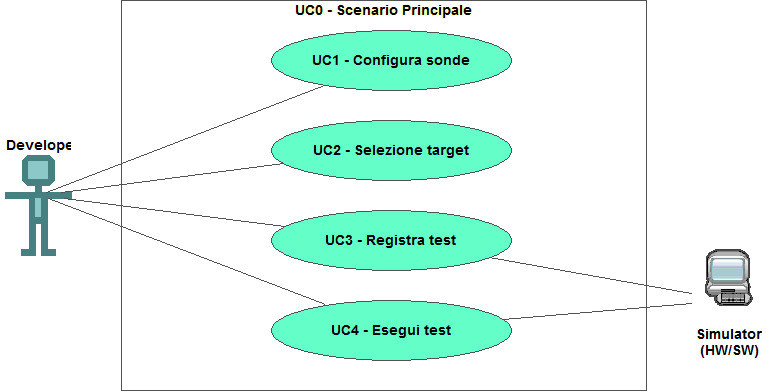
\includegraphics[alt={Testo alternativo dell'immagine}, width=0.75\columnwidth]{img/usecase/scenario-principale.jpeg}
    \caption{Use Case 0: Scenario principale}
    \label{fig:scenario_principale}
\end{figure}

\begin{usecase}{0}{Scenario principale}
    \usecaseactors{Sviluppatore applicativi.}
    \usecasepre{Lo sviluppatore è entrato nel plugin di simulazione all'interno dell'IDE.}
    \usecasedesc{La finestra di simulazione mette a disposizione i comandi per configurare, registrare o eseguire un test.}
    \usecasepost{Il sistema è pronto per permettere una nuova interazione.}
    \label{uc:uc_scenario_principale}
\end{usecase}

\begin{usecase}{1}{Gestione Utente}
    \usecaseactors{Amministratore, Utente Registrato.}
    \usecasepre{L'utente deve essere autenticato nel sistema.}
    \usecasedesc{L'utente può gestire le informazioni del proprio profilo.}
    \usecasepost{Le modifiche vengono salvate nel sistema.}
    \usecasealt{Se l'utente non è autenticato, visualizza un messaggio di errore.}
    \label{uc:uc_casi_uso}
\end{usecase}

\begin{usecase}{2}{Creazione Prodotto}
    \usecaseactors{Amministratore.}
    \usecasepre{L'amministratore ha effettuato l'accesso al sistema.}
    \usecasedesc{L'amministratore può aggiungere un nuovo prodotto al catalogo.}
    \usecasepost{Il nuovo prodotto viene aggiunto con successo.}
    \usecasealt{Se i campi obbligatori non sono compilati, visualizza un messaggio di errore.}
    \label{uc:uc_creazione_prodotto}
\end{usecase}

\section{Tracciamento dei requisiti}
Da un'attenta analisi dei requisiti e degli use case effettuata sul progetto è stata stilata la tabella che traccia i requisiti in rapporto agli use case.\\
Sono stati individuati diversi tipi di requisiti e si è quindi fatto utilizzo di un codice identificativo per distinguerli.\\
Il codice dei requisiti, dove ogni requisito è identificato con il carattere \textbf{R}, è così strutturato:
\begin{enumerate}
    \item[\textbf{F}:] Funzionale.
    \item[\textbf{Q}:] Qualitativo.
    \item[\textbf{V}:] Di vincolo.
    \item[\textbf{N}:] Obbligatorio (necessario).
    \item[\textbf{D}:] Desiderabile.
    \item[\textbf{Z}:] Opzionale.
\end{enumerate}

Nelle tabelle \ref{tab:requisiti_funzionali}, \ref{tab:requisiti_qualitativi} e \ref{tab:requisiti_vincolo} sono riassunti i requisiti e il loro tracciamento con gli use case delineati in fase di analisi.

\section{Tabelle dei requisiti}
\begin{center}
    \rowcolors{1}{}{tableGray}
    \begin{longtable}{|p{2.25cm}|p{7.75cm}|p{2.25cm}|}
    \hline
    %\rowcolor{hyperColor!5}
    \multicolumn{1}{|c|}{\textbf{Requisito}} & \multicolumn{1}{c|}{\textbf{Descrizione}} & \multicolumn{1}{c|}{\textbf{Use Case}}\\
    \hline 
    \endfirsthead
    \rowcolor{white}
    \multicolumn{3}{c}{{\bfseries \tablename\ \thetable{} -- Continuo della tabella}}\\
    \hline
    %\rowcolor{hyperColor!5}
    \multicolumn{1}{|c|}{\textbf{Requisito}} & \multicolumn{1}{c|}{\textbf{Descrizione}} & \multicolumn{1}{c|}{\textbf{Use Case}}\\
    \hline 
    \endhead
    \hline
    \rowcolor{white}
    \multicolumn{3}{|r|}{{Continua nella prossima pagina...}}\\
    \hline
    \endfoot
    \endlastfoot
    
    RFN-1 & L’interfaccia permette di configurare il tipo di sonde del test & UC1 \\
    \hline
    \hiderowcolors
    \caption{Tabella del tracciamento dei requisiti funzionali.}
    \label{tab:requisiti_funzionali}
    \end{longtable}
\end{center}

\begin{center}
    \rowcolors{1}{}{tableGray}
    \begin{longtable}{|p{2.25cm}|p{7.75cm}|p{2.25cm}|}
    \hline
    %\rowcolor{hyperColor!5}
    \multicolumn{1}{|c|}{\textbf{Requisito}} & \multicolumn{1}{c|}{\textbf{Descrizione}} & \multicolumn{1}{c|}{\textbf{Use Case}}\\
    \hline 
    \endfirsthead
    \rowcolor{white}
    \multicolumn{3}{c}{{\bfseries \tablename\ \thetable{} -- Continuo della tabella}}\\
    \hline
    %\rowcolor{hyperColor!5}
    \multicolumn{1}{|c|}{\textbf{Requisito}} & \multicolumn{1}{c|}{\textbf{Descrizione}} & \multicolumn{1}{c|}{\textbf{Use Case}}\\
    \hline 
    \endhead
    \hline
    \rowcolor{white}
    \multicolumn{3}{|r|}{{Continua nella prossima pagina...}}\\
    \hline
    %\caption{Tabella del tracciamento dei requisiti qualitativi.}
    \endfoot
    \endlastfoot
    
    RQD-1n & Le prestazioni del simulatore hardware deve garantire la giusta esecuzione dei test e non la generazione di falsi negativi & - \\
    \hline
    RQD-1n & Le prestazioni del simulatore hardware deve garantire la giusta esecuzione dei test e non la generazione di falsi negativi & - \\
    \hline
    RQD-1n & Le prestazioni del simulatore hardware deve garantire la giusta esecuzione dei test e non la generazione di falsi negativi & - \\
    \hline
    RQD-1n & Le prestazioni del simulatore hardware deve garantire la giusta esecuzione dei test e non la generazione di falsi negativi & - \\
    \hline
    RQD-1n & Le prestazioni del simulatore hardware deve garantire la giusta esecuzione dei test e non la generazione di falsi negativi & - \\
    \hline
    RQD-1n & Le prestazioni del simulatore hardware deve garantire la giusta esecuzione dei test e non la generazione di falsi negativi & - \\
    \hline
    \hiderowcolors
    \caption{Tabella del tracciamento dei requisiti qualitativi.}
    \label{tab:requisiti_qualitativi}
    \end{longtable}
\end{center}

\begin{center}
    \rowcolors{1}{}{tableGray}
    \begin{longtable}{|p{2.25cm}|p{7.75cm}|p{2.25cm}|}
    \hline
    %\rowcolor{hyperColor!5}
    \multicolumn{1}{|c|}{\textbf{Requisito}} & \multicolumn{1}{c|}{\textbf{Descrizione}} & \multicolumn{1}{c|}{\textbf{Use Case}}\\
    \hline 
    \endfirsthead
    \rowcolor{white}
    \multicolumn{3}{c}{{\bfseries \tablename\ \thetable{} -- Continuo della tabella}}\\
    \hline
    %\rowcolor{hyperColor!5}
    \multicolumn{1}{|c|}{\textbf{Requisito}} & \multicolumn{1}{c|}{\textbf{Descrizione}} & \multicolumn{1}{c|}{\textbf{Use Case}}\\
    \hline 
    \endhead
    \hline
    \rowcolor{white}
    \multicolumn{3}{|r|}{{Continua nella prossima pagina...}}\\
    \hline
    \endfoot
    \endlastfoot
    
    RVO-1 & La libreria per l'esecuzione dei test automatici deve essere riutilizzabile & - \\
    \hline
    \hiderowcolors
    \caption{Tabella del tracciamento dei requisiti di vincolo.}
    \label{tab:requisiti_vincolo}
    \end{longtable}
\end{center}

\newpage
    \chapter{Progettazione e codifica}
\label{chap:progettazione-codifica}
Breve introduzione al capitolo

\section{Tecnologie e strumenti}
\label{sec:tecnologie-strumenti}
Di seguito viene data una panoramica delle tecnologie e strumenti utilizzati.

\subsection*{Tecnologia 1}
Descrizione Tecnologia 1.

\subsection*{Tecnologia 2}
Descrizione Tecnologia 2

\section{Ciclo di vita del software}
\label{sec:ciclo-vita-software}

\section{Progettazione}
\label{sec:progettazione}

\subsection{Namespace 1}
Descrizione namespace 1.

\section{Design Pattern utilizzati}

\section{Codifica}
Blocco di codice in C
\begin{listing}[H]
\begin{minted}{c}
#include <stdio.h>
int main() {
    print("Hello, world!");
    return 0;
}
\end{minted}
\caption{Example of code}
\label{listing:c}
\end{listing}

\newpage
    \chapter{Verifica e validazione}
\label{chap:verifica-validazione}

\begin{figure}[H]
    \centering
    
\includegraphics[alt={Testo alternativo dell'immagine}, width=1\columnwidth]{img/quantum_superposition.jpeg}
    \caption{Lorem}
    \label{fig:enter-label}
\end{figure}

\lipsum[1-2]

% Esempio di come importare un file contenente codice
Lorem ipsum:
\begin{listing}[H]
\inputminted{python}{code/example.py}
\caption{Fibonacci recursive}
\label{listing:py_fibo}
\end{listing}

\lipsum[1]

\newpage
    \chapter{Conclusioni}
\label{chap:conclusioni}

\section{Consuntivo finale}
Esempio di aggiunta di un termine con glossario e acronimo:\\
Lorem \gls{sdk} ispum dolor.

Nel successivo utilizzo, apparirà solo l'acronimo:\\
Lorem \gls{sdk}.

Nel caso si voglia invece mettere solo il termine per esteso, si può usare:\\
Lorem \gls{sdkg}.

\section{Raggiungimento degli obiettivi}
Esempio di termine con solo acronimo\\
Lorem \gls{tsa}, ipsum dolor sit amet

termine costruito senza acronimo:
Lorem \gls{TermineSenzaAcronimo}, ipsum dolor sit amet

\section{Conoscenze acquisite}
Lorem Ipsum dolor Lorem \gls{api}

Lorem Ipsum dolor Lorem \gls{apig}

Si può consultare il file \textit{glossary\_acronyms.tex} per alcuni esempi.

\section{Valutazione personale}


\section{Valutazione personale}


\newpage

    \pagenumbering{roman}
    \backmatter
    \chapter{Bibliografia}
\label{cap:bibliography}

\nocite{*}

% Books bibliography
\printbibliography[heading=subbibliography, title={Testi}, type=book]

% Articles bibliography
\printbibliography[heading=subbibliography, title={Articoli}, type=article]

% Websites bibliography
%\printbibliography[heading=subbibliography, title={Siti}, type=online]

    \chapter{Sitografia}
\label{cap:webliography}
\nocite{*}

% Websites bibliography
\printbibliography[heading=subbibliography, title={\null}, type=online]

\end{document}